\scanpage{9}
$W$ vecteurs de Witt

$\Lambda_0\cdots\Lambda_\nu$ indéterminées, \unsure{liées|liés} par
\[
\left\{\begin{aligned}
\Lambda_i^p&=\frac{p^{i+1}!}{(p^i!)^p}\Lambda_{i+1}\qquad\text{si }0\leq i\leq\nu-1\\
\Lambda_\nu^p&=0
\end{aligned}\right.
\]
Ceci implique
\[
\Lambda_0^{a_0}\cdots\Lambda_\nu^{a_\nu}=0\quad\text{si }\sum a_ip^i\geq p^{\nu+1}\qquad(a_i\geq0
\]
\deleted{\unsure{Comme}} \uline{Dém} \figure{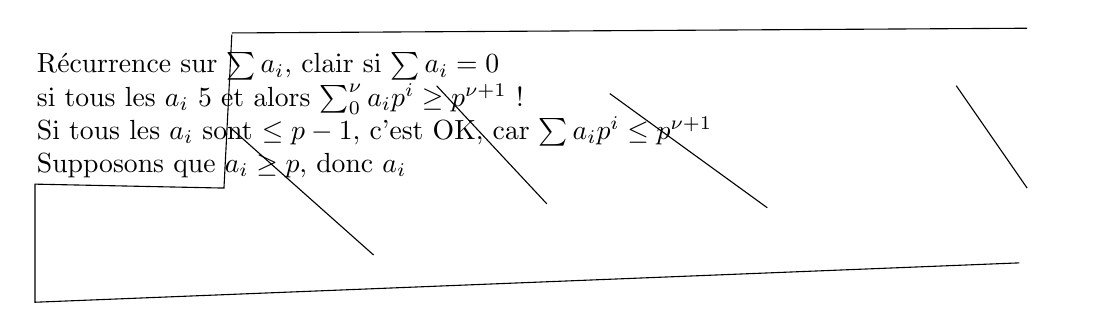
\begin{tikzpicture}[x=1cm,y=1cm]
\node[anchor=north west,text width=13cm,align=left] at (0,0) {\deleted{Récurrence sur $\sum a_i$, clair si $\sum a_i=0$\par si tous les $a_i$ \illegible{5} et alors $\sum_0^\nu a_ip^i\geq p^{\nu+1}$ !\par Si tous les $a_i$ sont $\leq p-1$, c'est OK, car $\sum a_ip^i\leq p^{\nu+1}$\par Supposons que $a_i\geq p$, \unsure{donc} $a_i$}};
\draw (2.6,.12)--(12.7,.18);
\draw (2.6,.1)--(2.5,-1.85)--(.1,-1.8)--(.1,-3.3)--(12.6,-2.8);
\draw (2.6,-1.1)--(4.4,-2.7);
\draw (5.2,-.55)--(6.6,-2.05);
\draw (7.4,-.65)--(9.4,-2.1);
\draw (11.8,-.55)--(12.7,-1.85);
\end{tikzpicture}}

\deleted{\unsure{si}} \deleted{\unsure{est}}

\uline{Lemme}
\[
\Lambda_0^{a_0}\Lambda_1^{a_1}\cdots\Lambda_\nu^{a_\nu}=c\Lambda_0^{b_0}\cdots\Lambda_{\nu-1}^{b_{\nu-1}}\Lambda_\nu^{b_\nu},\qquad c\in W
\]
avec $0\leq b_\alpha\leq p-1$ pour $0\leq i\leq\uline{\nu-1}$ et $b_\nu$ a priori \unsure{qq.}, et
\[
\sum_0^\nu a_ip^i=\sum_0^\nu b_ip^i
\]
Pour le voir, on \deleted{procède} par récurrence, \deleted{\unsure{sur} $\sum a_i$, \unsure{de sorte}} \inserted{transformons} l'expression en une expression $c\Lambda_0^{a'_0}\cdots\Lambda_\nu^{a'_\nu}$, avec les $a'_\alpha\leq p-1$.
\deleted{\unsure{par} $\sum a_i$, \unsure{puis tous} $a_i$ \unsure{tels}} \inserted{\unsure{le premier des} $a'_\alpha\leq p-1$}
\deleted{Donc \unsure{pour} $\sum a_i$, \unsure{si on a}} \inserted{$\alpha\leq p-1\ (i\leq\nu-1)$}
Si \unsure{nous} (pour $a_i$ \deleted{$\unsure{(i\leq\nu-1)}$} est $\geq p$, on écrit $a_i=pq_i+a'_i$, d'où
\[
\Lambda_i^{a_i}=(\Lambda_i^p)^{a'_i}\Lambda_i^{\alpha_i}=(c_i\Lambda_{i+1})^{a'_i}\Lambda_i^{\alpha_i}=c'\Lambda_{i+1}^{a'_i}\Lambda_i^{\alpha_i}
\]
donc
\[
\Lambda_0^{a_0}\cdots\Lambda_\nu^{a_\nu}=c\Lambda_0^{a_0}\cdots\Lambda_i^{a'_i}\Lambda_{i+1}^{\overbrace{a_{i+1}+q_i}^{\inserted{a'_{i+1}}}}\Lambda_{i+2}^{a_{i+2}}\cdots,
\]
et évidemment on a
\[
\sum a_ip^i=\sum a'_ip^i,
\]
car
\[
\deleted{a'_ip^i+}\quad\underline{a'_ip^i+\underline{(a_{i+1}+q_i)}}p^{i+1}=\underbrace{(a'_i+q_ip)}_{a_i}p^i+a_{i+1}p^{i+1}.
\]
Or, si on a $\sum b_ip^i\geq p^{\nu+1}$, alors \deleted{\unsure{on}} (et alors seulement) \deleted{$\unsure{p}$} $b_\nu\geq p$, donc $\Lambda_\nu^{b_\nu}$ est un \deleted{\unsure{multiple de} $\unsure{\Lambda_\nu^p}$} multiple de $\Lambda_\nu^p$, or $\Lambda_\nu^p=0$. OK.
\mspage{8}
